\section{Model Comparison Results}

This section presents the final empirical comparison. The main result is that LSTM-attention is the strongest model in the current pipeline. It outperforms the earlier baselines and gives the best downstream trading result among the tested architectures.

\begin{figure}[H]
    \centering
    \begin{subfigure}[t]{0.82\linewidth}
        \centering
        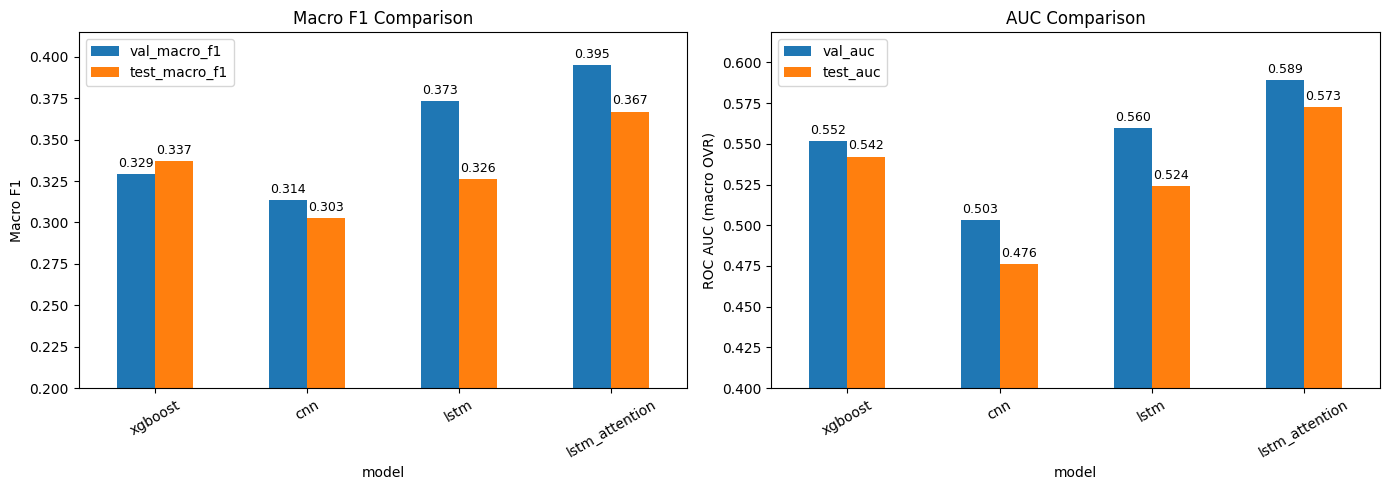
\includegraphics[width=\linewidth]{figures/metrics_across_4_models.png}
        \caption{Model metrics.}
    \end{subfigure}

    \vspace{0.35em}

    \begin{subfigure}[t]{0.72\linewidth}
        \centering
        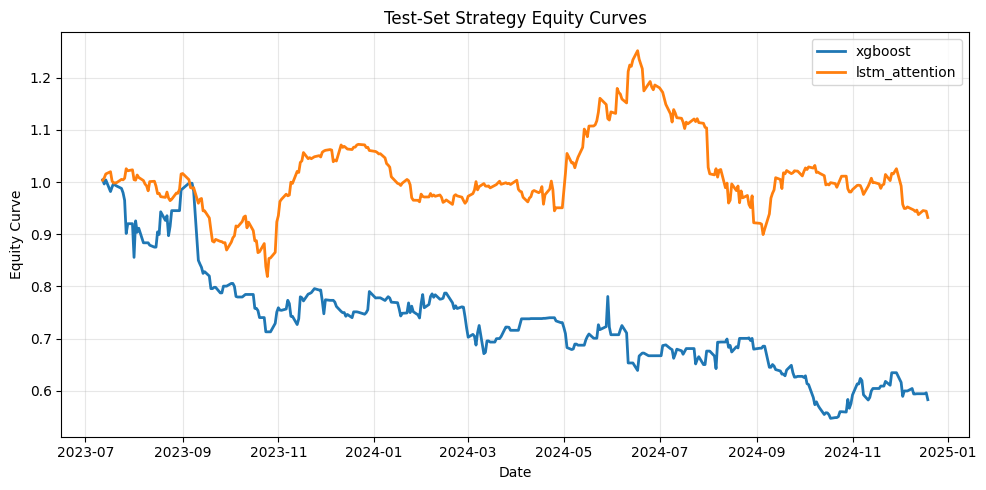
\includegraphics[width=\linewidth]{figures/lstm_attention_vs_xgboost_equity.png}
        \caption{Equity comparison.}
    \end{subfigure}
    \caption{Compact summary of the final results.}
\end{figure}

The metric comparison shows the overall ranking across architectures. XGBoost remains a strong baseline, CNN does not add enough value, and the plain LSTM still does not surpass the tree baseline. The best result comes from LSTM-attention, which supports the claim that cross-sectional interaction is the missing piece.

The final equity comparison is the most important result: the gain from LSTM-attention is not only visible in classification metrics, but also appears in downstream trading performance relative to XGBoost.
